\chapter{DEFINICIÓN DEL PROBLEMA}
\label{chapter:problem}
\hyphenation{BeamCal}
En esta tesis de pre-grado se describe el diseño y la implementación de una plataforma de pruebas cuyo fin es poder someter a pruebas y caracterizar a the bean V2, un integrado de aplicación específica para satisfacer las necesidades de instrumentación del BeamCal, un detector del International Linear Collider.

\section{El colisionador lineal internacional}
El ILC es un colisionador de partículas aún  en etapa de diseño, que pretende complementar los descubrimientos realizados por el LHC en el 2012. Este instrumento colisionará electrones contra sus  anti-partículas los positrones, para lo cual cuenta principalmente de dos aceleradores los que comprenden una extension de aproximadamente 31 kilómetros. En estos aceleradores las partículas confinadas dentro de un haz son aceleradas por medio de campos electromagnéticos hasta alcanzar velocidades relativas a la velocidad de la luz, para luego ser colisionadas. La escala de energía en estas colisiones serán del orden de 500 GeV para su primera etapa. Posteriormente en una segunda etapa, el ILC contempla actualización que pretende utilizar una estructura de aceleradores de 50 kilómetros y niveles de energía de 1 Tev. Estos representan niveles de energía nunca antes observados en la tierra, es por esta razón que estos aceleradores reciben el nombre de aceleradores de ``escala tera". 

El proyecto del ILC representa un desafío de carácter mundial. Más de 300 laboratorios y Universidades de todo el mundo participan en el diseño de este nuevo instrumento de alto nivel para la física de partículas.  Debido a que tanto la realización de un proyecto de esta magnitud, así como las tareas de coordinación representan un desafío extremadamente complejo, muchas de las especificaciones que comprenden al proyecto aun están en discusión. Un ejemplo de esto es el emplazamiento de este proyecto, el cual aun no se encuentra definido.


\section{El detector frontal y the BeamCal}
En un acelerador de partículas las colisiones se llevan a cabo dentro de un gran detector, el cual esta a su vez compuestos de un conjunto de distintos detectores, destinados a medir fenómenos específicos, los cuales a su vez se encuentran altamente segmentados. La estructura de estos detectores para el ILC aun permanece en estudio, sin embargo, existen dos propuestas validadas como candidatas. Cada una de estas propuestas considera la presencia de un detector frontal en su estructura. El propósito de este detector frontal es realizar mediciones de la luminosidad de alta velocidad y precisión, y asegurar la hermiticidad del detector.

Para lograr dichas tareas, el detector frontal cuenta a su vez con dos calorímetros principales ubicados en las capas más cercanas al haz de partículas: el LumiCal y el BeamCal.
The BeamCal es un calorímetro electromagnético altamente segmentado,  adyacente al haz de partículas y cuenta principalmente con tres propósitos: Mejorar la hermeticidad del ILC para ángulos polares bajos, reducir el backscattering para pares en la parte interior del detector del ILC y asistir al diagnostico del haz de partículas. Las especificaciones del BeamCal para la tolerancia de radiación, ruido, carga de señal, tasas de pulsos y tiempos de ocupación plantean un reto único para el sistema de instrumentación. 

\section{The bean}
En este contexto se enmarca The bean V2, un IC que implementa un prototipo para la segunda iteración de The bean, el cual es un ASCI de 32 canales que implementará el front-end  para un detector destinado a formar parte de BeamCal. 

\begin{figure}[!t]
	\centering
	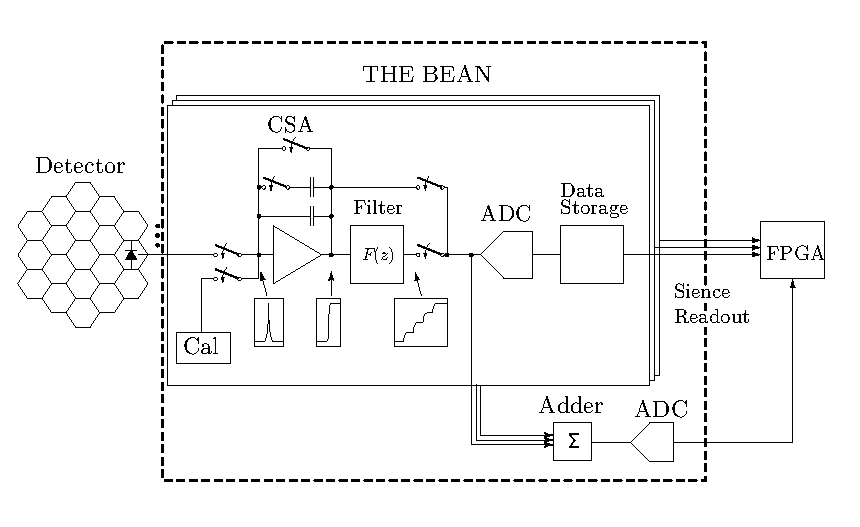
\includegraphics[width=5in]{./figures/thebeamdiagram-02.eps}
	\caption{Diagrama de bloques de The bean.}\label{fig:thebean_diagram}
\end{figure}

Cada canal de la versión final de The bean incluirá: un amplificador sensible a la carga con un pulsador de pre-carga; un filtro de capacitores conmutados (SC) totalmente diferencial con características de supresión de bajo ruido; un conversor análogo-digital(ADC) totalmente diferencial de aproximación sucesiva de 10 bits; y sistema para almacenar la información de salida, ya sea en una memoria analógica o digital. Adicionálmente, el IC cuenta con una red de feed-back para propósitos de diagnostico. En la figura \ref{fig:thebean_diagram} se entrega un diagrama de la estructura de The bean. 
 
El IC debe ser capaz de procesar la información proveniente del detector BeamCal a una frecuencia nominal de 3.2468 MHz, con un 100\% de ocupación. Por otro lado, cada canal debe ser capas de lidear con dos modos diferentes de operación: El modo de adquisición estandar ( standar data taking mode o SDT mode) y el modo de calibración del detector (Detector Calibration mode o DCal mode). Según las especificaciones de BeamCal, la máxima señal de entrada corresponde aproximadamente a $37pC$ en el modo SDT  y 50 veces menor en el modo DCal.
Por otro lado, dada la proximidad del detector a las colisiones, este esta expuesto a granes cantidades de radiación (1Mrad $\text{SiO}_2$).

\begin{table}[!h]
	\begin{center}
		\begin{tabular}{|l|l|}\hline
			Input rate & $3.25\,\text{MHz}$ during $0.87\,\text{ms}$, repeated every $200\,\text{ms}$ \\ \hline
			Channels per ASIC & $32$ \\ \hline
			Occupancy & $100\%$ \\ \hline
			Resolution & $10$ bits for individual channels, $8$ bits for fast feedback \\ \hline
			Modes of operation & Standard data taking (SDT), Detector Calibration (DCal) \\ \hline
			Input signals & Up to $40$ pC in SDT, $0.74$ pC in DCal \\ \hline
			Input capacitance & $65$ pF \\ \hline
			Additional feature & Low-latency ($1\,\micro\text{s}$) output \\ \hline
			Additional feature & Internal pulser for electronics calibration \\ \hline
			Radiation tolerance & 1 Mrad ($\text{SiO}_2$) total ionizing dose \\ \hline
			Power consumption & $2.19$ mW per channel \\ \hline
			Total ASIC count & $2836$ \\\hline
		\end{tabular}
		\vspace*{5pt}
		\caption{Resumen de las especificaciones para el ASIC de instrumentación para the BeamCal.}\label{tab:bean_specs}
	\end{center}
\end{table}

 La tabla \ref{tab:bean_specs} resume las especificaciones a las que esta sometido el IC the bean, las cuales son heredadas de los requisitos exigidos por the BeamCal.


\section{La plataforma de pruebas}
El desafío del trabajo presentado en esta tesis de pre-grado consiste en lograr implementar una plataforma que permita poder instanciar todas las condiciones necesarias para poder probar el funcionamiento del integrado the bean V2. En la figura \ref{fig:thebean_spec} se presenta la estructura general de las señales que intervienen en el IC.
Esta investigación se realizó bajo el patrocinio de CONICYT a través del programa FONDECYT.
El FONDECYT  \# 1110165: Aplicación de técnicas CMOS avanzadas en el procesamiento de pulsos para experimentos en física de partículas.

AGREGAR:

en este trabajo se llevó a cabo una segunda iteración de the Bean. Los principales resultados de esta investigacion son la implementan de una nueva metodologia de analisis para el ruido de los fornt ends de detectores de particulas basados en un análisis en el dominio del tiempo. El resultado principal consiste en que las ecuaciones para caracterizar el ruido son en general complejas en el dominio del tiempo. sin embargo 





Debido a que The bean V2 es un integrado de señales mixtas este requiere de alimentación analógica y digital. Ambas alimentaciones deben ser de $1.8V$ y de bajo ruido. Las entradas del circuito se dividen en entradas analógicas y digitales. Las entradas analógicas son: una señal de entrada para uno de los canales del front-end, y una entrada diferencial para un el filtro de prueba.  Las entradas digitales, representan todas las señales de control, que periten definir el modo de operación del IC y controlan su funcionamiento. Por otra parte, las salidas del IC corresponden a voltajes analógicos, los cuales son: un par de salidas provenientes desde buffers para seguimiento del funcionamiento del integrado; un par de salidas diferenciales provenientes desde el filtro de prueba; y un par diferencial correspondiente a la salida del canal del front-end. Junto con las señales descritas, el integrado necesita de un grupo de voltajes analógicos, los cuales definen el punto de operación del integrado. En la sección \ref{chapter:theoretical} se entrega un estudio más detallado del funcionamiento de cada una de las señales del integrado. 

\begin{figure}[!t]
	\centering
	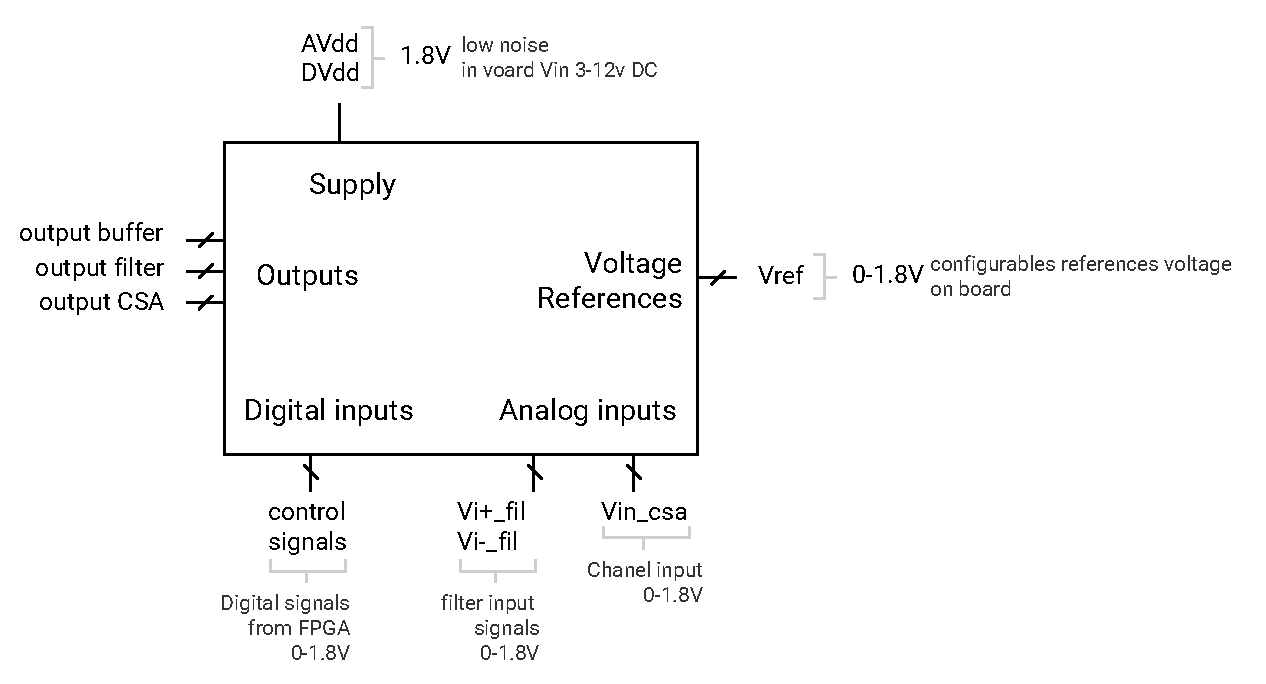
\includegraphics[width=5in]{./figures/especificiaciones-01}
	\caption{Diagrama general de los requisitos del IC.}\label{fig:thebean_spec}
\end{figure}



Para generar el control de las variables digitales, la plataforma de pruebas debe contar con una interfaz que permita comunicarse con un control digital. Dadas las especificaciones del problema, desarrollar un control basado en una FPGA aparece como la mejor opción. Dado la versatilidad que ofrecen las FPGAs, es posible desarrollar un control tan específico como sea necesario. Además las FPGA comúnmente cuentan con un gran número de pines I/O lo cual permitiría controlar múltiples señales de controles de forma paralela, aumentando la velocidad de procesamiento.

Otro de los aspectos importantes a considerar en los requisitos para la plataforma de pruebas, es la capacidad de operar \textit{on-line}, es decir, poder realizar continuas iteraciones de secuencias de entradas para distintas configuraciones y condiciones de operación del integrado, sin tener que re-programar la FPGA. Esto implica contar con un protocolo que permita establecer una comunicación entre un computador y el control en la FPGA.

En resumen la plataforma de pruebas a implementar debe cumplir con los siguientes requisitos:
\begin{itemize}
\item Contar con reguladores de voltaje para generar la alimentación del IC the bean V2.
\item Poseer la capacidad de generar distintos voltajes para emular las entradas necesarias del sistema, lo cual debe implementarse en base a un conversor digital análogo (DAC) de 12 bits.
\item Debe contar con la capacidad de leer los datos de salida, para esto es necesario contar con dos conversores análogo digital (ADC) de 10 bits totalmente diferenciales.
\item  Debe poder ser capaz de generar los voltajes de referencia para poder ajustar el punto de operación del integrado.
\item Implementar una interfaz que permita comunicarse directamente con un control digital en una FPGA.
\item Implementar junto al control un protocolo de comunicación FPGA-Computador, que permita el control \textit{on-line} del integrado.
\end{itemize}


Finalmente los objetivos específicos del trabajo presentado en esta tesis de pre-grado son:
\begin{enumerate}
\item Implementar una plataforma de pruebas que permita caracterizar bajo parámetros definidos un circuito integrado especifico llamado The bean V2.
\item Implementar dentro de la misma plataforma la capacidad de operar on-line.
\item Caracterizar el integrado dentro de las pruebas y parámetros establecidas bajo las consideraciones expuestas en este trabajo.
\end{enumerate}